\documentclass[11pt]{article}
\usepackage[scaled=0.92]{helvet}
\usepackage{geometry}
\geometry{letterpaper,tmargin=1in,bmargin=1in,lmargin=1in,rmargin=1in}
\usepackage[parfill]{parskip} % Activate to begin paragraphs with an empty line rather than an indent %\usepackage{graphicx}
\usepackage{amsmath,amssymb, mathrsfs,  mathtools, dsfont}
\usepackage{tabularx}
\usepackage[font=footnotesize,labelfont=bf]{caption}
\usepackage{graphicx}
\usepackage{xcolor}
%\usepackage[linkbordercolor ={1 1 1} ]{hyperref}
%\usepackage[sf]{titlesec}
\usepackage{natbib}
\usepackage{../../Tianpei_Report}


\begin{document}
\title{Self-study: The geometry of exponential families}
\author{ Tianpei Xie}
\date{ Jun. 1st., 2015 }
\maketitle
\tableofcontents
\newpage
\section{The statistical manifold and the exponential families}
\subsection{Concepts}
\begin{itemize}
\item A \emph{\textbf{statistical manifold}} \citep{murray1993differential, amari2007methods}: Any parametrised family of probability distributions,
\begin{align*}
\cP &= \set{p(\mb{x}; \mb{\theta})} 
\end{align*}
with parameter $\mb{\theta}$ running over some open subset of $\bR^d$ , is automatically a \emph{\textbf{manifold}}, in which the probability distributions are the points of the manifold and the parameters are co-ordinate functions. 

\item \begin{definition}
Let $p$, $q$ be $\bR^d \supset \cM_{0}: \rightarrow  \bR$ density functions and let $\alpha \in \bR \setminus \set{1}$. The \emph{\textbf{R\'enyi divergence}} of order $\alpha$ or \underline{\textbf{$\alpha-$divergence}} of a distribution $p$ from a distribution $q$ is defined to be 
\begin{align}
\divg{\alpha}{p}{q} &= \frac{1}{\alpha -1}\log\brac{\E{Q}{\paren{\frac{dP}{dQ}}^{\alpha}}}  = \frac{1}{\alpha -1}\log\paren{\int_{ \cM_{0}}p^{\alpha}(x)q^{1-\alpha}(x)\;  \mu(dx)} \label{eqn: alpha_divg}
\end{align} 
\end{definition}

\item   \begin{definition}
Let $P$ and $Q$ be two probability distributions over a space $\Omega$, such that  $P\ll Q$, that is, $P$ is \emph{\textbf{absolutely continuous}} with respect to $Q$. Then, for a \underline{\emph{\textbf{convex function}}}  $f: [0, +\infty)\to (-\infty ,+\infty]$ such that $f(x)$ is finite for all $x>0$, \underline{$f(1)=0$}, and  \underline{$f(0)=\lim _{t\to 0^{+}}f(t)$} (which could be infinite), the \underline{\emph{\textbf{f-divergence}}} of $P$ from $Q$ is defined as
\begin{align}
\divg{f}{P}{Q} &= \E{Q}{f\paren{\frac{dP}{dQ}}} =  \int_{\Omega} f\paren{\frac{dP}{dQ}} dQ  =  \int_{\Omega} q(x) f\paren{\frac{p(x)}{q(x)}} \mu(dx)  \label{eqn: f_divg}
\end{align}
\end{definition}
\end{itemize}

\subsection{Exponential families}
\begin{itemize}
\item The canonical representation of \underline{\emph{\textbf{exponential famlity}}} of distribution has the following form
\begin{align}
p(x_1, \ldots, x_{m}) = p(\mb{x}; \mb{\eta}) &= \exp\paren{\inn{\mb{\eta}}{\mb{\phi}(\mb{x})} - A(\mb{\eta})}\mu(d\mb{x}) \nonumber \\
&= \exp\paren{\sum_{i=1}^{d}\eta_{i}\phi_{i}(\mb{x}) -  A(\mb{\eta})}\mu(d\mb{x}) \label{eqn: exp_fam}
\end{align} where $\phi$ is a feature map  and $\mb{\phi}(\mb{x})$ defines a set of \emph{\textbf{sufficient statistics}} (or \emph{\textbf{potential functions}}). The normalization factor is defined as
\begin{align*}
 A(\mb{\eta}) &:= \log \int \exp\paren{ \inn{\mb{\eta}}{\mb{\phi}(\mb{x})} }h(\mb{x})\nu(d\mb{x}) = \log Z(\mb{\eta})
\end{align*} $A(\mb{\eta})$ is also referred as \textbf{\emph{log-partition function}} or \emph{cumulant function}. The parameters $\mb{\eta} = (\eta_{\alpha})$ are called \textbf{\emph{natural parameters}}  or \emph{canonical parameters}. The canonical parameter $\set{\eta_{\alpha}}$ forms a \textbf{natural (canonical) parameter space}
\begin{align}
\Omega = \set{\mb{\eta} \in \bR^{d}: A(\mb{\eta}) < \infty} \label{eqn: canonical_space}
\end{align}

\item The exponential family is the unique solution of \textbf{\emph{maximum entropy estimation}} problem:
\begin{align}
\min_{q \in \Delta}&\quad \kl{q}{p_{0}} \label{eqn: max_ent}\\
\text{s.t.}&\quad \E{q}{\phi_{\alpha}(X)} = \mu_{\alpha}\,\quad  \forall\, \alpha \in \cI   \label{eqn: max_ent_mean_constraint}
\end{align} where $\kl{q}{p_0} = \int \log(\frac{q}{p_0}) q dx = \E{q}{\log\frac{q}{p_0}}$ is the relative entropy or the Kullback-Leibler divergence of $q$ w.r.t. $p_0$.

Here $\mb{\mu} = (\mu_{\alpha})_{\alpha \in \cI}$ is a set of  \textbf{\emph{mean parameters}}. The space of mean parameters $\cM$ is a \emph{convex polytope} spanned by potential functions $\set{\phi_{\alpha}}$.
\begin{align}
\cM &:= \set{\mb{\mu} \in \bR^d: \exists q\,\; \text{s.t. } \E{q}{\phi_{\alpha}(X)} = \mu_{\alpha}\,\quad  \forall\, \alpha \in \cI} = \text{conv}\set{\phi_{\alpha}(x),\; x\in \cX, \;\alpha \in \cI}  \label{eqn: marginal_polytope}
\end{align}

\item Note that $A(\mb{\eta})$ is a convex function and its gradient $\grad{}{A}: \Omega \rightarrow \cM^{\circ}$ is a bijection between the natural parameter space $\Omega$ and the \underline{\textbf{interior}} of $\cM$,  $\cM^{\circ}$; $\grad{}{A}(\mb{\eta}) = \mb{\mu}$ based on the following equation 
\begin{align}
\partdiff{A}{\eta_{\alpha}} &= \E{\mb{\eta}}{\phi_{\alpha}(X)} := \int_{\cX^{m}}\phi_{\alpha}(\mb{x}) q(\mb{x}; \mb{\eta}) d\mb{x} = \mu_{\alpha} \label{eqn: partition_first_order}
\end{align}

\item Moreover $A(\mb{\eta})$ has a variational form 
\begin{align}
A(\mb{\eta}) &=  \sup_{\mb{\mu} \in \cM}\set{ \inn{\mb{\eta}}{\mb{\mu}} - A^{*}(\mb{\mu})} \label{eqn: log_partition_variational_form}
\end{align}
where $A^{*}(\mb{\mu})$ is the conjugate dual function of $A$ and it is defined as
\begin{align}
A^{*}(\mb{\mu}) &:= \sup_{\mb{\eta} \in \Omega} \set{\inn{\mb{\mu}}{\mb{\eta}} - A(\mb{\eta})} \label{eqn: conjugate_dual_partition}
\end{align}

It is shown that $A^{*}(\mb{\mu})  = -H(q_{\mb{\eta}(\mb{\mu})})$ for $\mb{\mu} \in  \cM^{\circ}$ which is the negative entropy. $A^{*}(\mb{\mu})$ is also the optimal value for the \textbf{maximum likelihood estimation} problem on $p$. The exponential family can be reparameterized according to its mean parameters $\mb{\mu}$ via backward mapping $(\grad{}{A})^{-1}: \cM^{\circ} \rightarrow  \Omega$, called \textbf{mean parameterization}.

\item The \emph{gradient of log-likelihood function} (\emph{\textbf{score functions}}) for exponential family is 
\begin{align}
\grad{\mb{\eta}}{\log p(\mb{x}; \mb{\eta})} &= \mb{\phi}(\mb{x}) - \grad{\mb{\eta}}{A(\mb{\eta})} = \mb{\phi}(\mb{x}) - \E{p}{\mb{\phi}(\mb{X})} \label{eqn: score_function_exp_fam}
\end{align}

\item The \emph{\textbf{Fisher information}} for exponential family is 
\begin{align}
[\mb{I}(\mb{\eta})]_{i,j} &:= \E{\mb{\eta}}{\paren{\partdiff{}{\eta_{i}}\log p(\mb{x}; \mb{\eta})}\paren{\partdiff{}{\eta_{j}} \log p(\mb{x}; \mb{\eta})}} \nonumber\\
&= -\E{\mb{\eta}}{\frac{\partial^2 }{\partial \eta_{i} \partial \eta_{j}} \log p(\mb{x}; \mb{\eta}) } \label{eqn: fisher_information}\\
&= \frac{\partial^2 A(\mb{\eta})}{\partial \eta_{i} \partial \eta_{j}} =\E{\mb{\eta}}{\phi_{i}(\mb{X})\phi_{j}(\mb{X})} -  \E{\mb{\eta}}{\phi_{i}(\mb{X})} \E{\mb{\eta}}{\phi_{j}(\mb{X})}\label{eqn: fisher_information_partition_second_order} \\
&:= \text{Cov}(\phi_{i}(\mb{X}), \phi_{j}(\mb{X})) \nonumber
\end{align}
Note that $A(\mb{\eta})$ is convex, so the Fisher information matrix is positive definite $\mb{I}(\mb{\eta}) \succ \mb{0}$.

%The Fisher information matrix is of paramount importance in parametric statistical theory and lies at the heart of flnite and large sample optimality theory in statistical inference problems for general regular parametric families.

%\item We can formulate the \textbf{KL divergence} between two distributions in exponential family $\Omega$ using its primal and dual form
%\begin{itemize}
%\item \textbf{Primal-form}: given $\mb{\eta}_1, \mb{\eta}_2 \in \Omega$
%\begin{align}
%\kl{p_{\mb{\eta}_1}}{p_{\mb{\eta}_2}} \equiv  \kl{\mb{\eta}_1}{\mb{\eta}_2}
%&=  A(\mb{\eta}_2) - A(\mb{\eta}_1) -  \inn{\mb{\mu}_{1}}{\mb{\eta}_2 - \mb{\eta}_1}  \label{eqn: kl_primal}\\
%&\equiv  A(\mb{\eta}_2) - A(\mb{\eta}_1) -  \inn{\grad{}{A}(\mb{\eta}_1)}{\mb{\eta}_2 - \mb{\eta}_1}  \nonumber
%\end{align}
%
%\item \textbf{Primal-dual form}: given $\mb{\mu}_1 \in \cM, \mb{\eta}_2 \in \Omega$
%\begin{align}
% \kl{\mb{\mu}_1}{\mb{\eta}_2} &= A(\mb{\eta}_2) + A^{*}(\mb{\mu}_1) - \inn{\mb{\mu}_{1}}{\mb{\eta}_2}  \label{eqn: kl_primal_dual}
%\end{align}
%
%\item \textbf{Dual-form}: given $\mb{\mu}_1, \mb{\mu}_2  \in \cM$
%\begin{align}
% \kl{\mb{\mu}_1}{\mb{\mu}_2} &= A^{*}(\mb{\mu}_1) - A^{*}(\mb{\mu}_{2}) - \inn{\mb{\eta}_2}{\mb{\mu}_{1} - \mb{\mu}_{2}}  \label{eqn: kl_dual} \\
% &\equiv  A^{*}(\mb{\mu}_1) - A^{*}(\mb{\mu}_{2}) - \inn{\grad{}{A^{*}}(\mb{\mu}_{2})}{\mb{\mu}_{1} - \mb{\mu}_{2}} \nonumber
%\end{align}
%\end{itemize}
\end{itemize}

\newpage
\section{The information geometry of exponential families}
\subsection{Information geometry and its related concepts}
The field of \underline{\emph{\textbf{information geometry}}} \citep{murray1993differential, amari2007methods} refers to an interdisciplinary field that applies the techniques of \emph{\textbf{differential geometry}} \citep{do1976differential, do1992riemannian, lee2003introduction} to study   \emph{\textbf{families of probability distributions and statistics}}.

Statistical inference concerns situations in which one knows or suspects that data are generated by sampling from a space according to a probability distribution which is a member of some known family $p(\theta)$.  The problem is to infer facts about the distribution from the data. For example, one might want to know the parameter value of the distribution (\emph{point estimation}), or simply whether or not this value lies in some \emph{particular set} of parameters (\emph{hypothesis testing}). 

There are several \textbf{motivations} to study \emph{information geometry}:
\begin{itemize}
\item Many of hypothesis tests and much of the theory of statistical inference depends on \textbf{\underline{the choice} of parameters}. It is important to know how the theory depends on the parameters, either because one suspects that \textbf{it should not depend on the parameters at all} or because one would like to know if a particular choice of parameters may \textbf{simplify} matters. Differential geometry provides tools to do "\emph{\textbf{calculus on manifolds}}".

\item In information geometry, we think of \underline{\textbf{\emph{families of probability distributions}}} as \emph{entities} \underline{\emph{\textbf{independent}}} of any particular \underline{\emph{\textbf{parametrization}}}, and able to  support a variety of \emph{\textbf{geometries}}. Information geometry involves studies of \underline{\emph{\textbf{invariants}}} under certain transformation on distributions

\item In information geometry, we relate the \underline{\emph{\textbf{statistical properties}}} to the  \emph{\textbf{geometries}} of underlying space of probablity distributions.
\end{itemize}

We listed concepts in information geometry as follows: 
\begin{itemize}
\item From \underline{\textbf{differential geometry}}: 
\begin{itemize}
\item \emph{\textbf{manifold}}, \emph{sub-manifold}, \emph{affine subspace},   \emph{diffeomorphism}, \emph{coordinate systems}, \emph{differential form}, \emph{differential operator},
\item \emph{tangent space}, \emph{(tangent) vector field},  \emph{change of coordinates},  \emph{Christoffel symbols},  \emph{Gauss map},  \emph{The first and second fundamental form of a regular surface},   
\item  \emph{curvature}, \emph{\textbf{Riemannian metric}}, \emph{\textbf{isometry}}, \emph{intrinsic geometry of a surface}, 
\item  \emph{covariant derivative}, \emph{\textbf{parallel transport}}, \emph{parallel translation}, \emph{\textbf{geodesics}}, \emph{exponential map}, \emph{\textbf{connection}}, \emph{affine connection}, \emph{\textbf{Riemannian connection}}, \emph{dual connection}, 
\end{itemize}

\item From \underline{\textbf{statistics and information theory}}: 
\begin{itemize}
\item \emph{parameterization},  \emph{\textbf{log-likelihood}}, \underline{\emph{\textbf{Fisher information metric}}},  \emph{sufficient statistics}, \emph{\textbf{exponential families}}, \emph{log-partition functions/cumulant functions}, \emph{maximum likelihood estimator}, \emph{maximum entropy estimator}, \emph{Cram\'er-Rao inequality}, \emph{asymptotics} 
\item  \emph{entropy}, \underline{\emph{\textbf{statistical divergences}}}, \emph{KL divergence}, \emph{R\'enyi divergence}, \emph{f-divergence}, \emph{Wasserstein distance}, 
%\item \emph{exponential-connection}, \emph{mixture-connection}, \emph{duality of connections}, 
\end{itemize}
\end{itemize}


\subsection{Affine spaces}
\begin{itemize}
\item An affine space is nothing more than a \emph{vector space} whose \textbf{origin} we try to forget about, by adding \textbf{translations} to the linear maps.  In an affine space, there is \emph{\textbf{no} distinguished point} that serves as an \emph{\textbf{origin}}.  Hence, no vector has a fixed origin and no vector can be uniquely associated to a point.

\item \begin{definition}
 An \emph{\textbf{affine space}} is defined as a set $X$ together with a \emph{\textbf{vector space}} $V$  and a \emph{transitive} and \emph{free action} of the \emph{\textbf{additive group}} of $V$ on $X$. Explicitly, we define the \emph{\textbf{translation}} action $+: X \times V \rightarrow X$, so that $(p,v) \mapsto p + v$.  The translation  have to satisfy the following rules
 \begin{enumerate}
 \item \emph{Right identity:} $a + 0 = a$ for any $a\in X$ and $0 \in V$ is the zero vector;
 \item \emph{Associativity:} $(p+ v) + w = p+ (v + w)$ for any point $p\in X$ and vectors $v, w \in V$;
 \item \emph{Subtraction:} given any two points $p, q \in X$ there must be a unique translation that moves one to the other, i.e. $q = p +  v$ for some unique $v \in V$
 \end{enumerate}
 \end{definition}
 
\item An affine space is a \emph{\textbf{principal homogeneous space}} for the action of the additive group of a vector space. The element of $X$ is called \emph{points} and the vector from the associated vector space $V$ is called \emph{free vectors}. The operation $p+v$ is called \emph{\textbf{translation by}} $v$ from $p$.
 
\item \begin{definition}
An \emph{\textbf{affine subspace}} of  $X$ is the subset of $X$ of the form 
 \begin{align*}
p + W =  \set{p + w \,|\, w \in W}
 \end{align*} where $p\in X$ and $W \subseteq V$ is a linear subspace of $V$ associated with $X$.
 \end{definition}
 
 \item The linear subspace associated with an affine subspace is often called its \emph{\textbf{direction}}, and two subspaces that \emph{share the same direction} are said to be \emph{\textbf{parallel}}. Every translation $A\to A: a\mapsto a+v$  maps any affine subspace to a parallel subspace.
 
%\item An \emph{affine space} can be thought of as a set $X$  which becomes a \emph{vector space} $V$ by selecting a point to be the zero point. 

%\item A vector in the affine space doesn't usually refer to a single arrow but rather to \emph{a whole family of arrows} which are \emph{\textbf{parallel translates}} of each other. In other words, we regard two arrows which are parallel translates of each other as instances of the same vector.


%\item Affine spaces have a fundamental geometic significance in that they are to be considered \emph{\textbf{fiat}}. A \emph{\textbf{characteristic}} of affine spaces is the presence of special \emph{coordinate systems} called \emph{affine coordinates}. 
\end{itemize}

\subsection{Log-likelihood and affine structure}
\begin{itemize}
\item \begin{definition}
Denote $\cM$ as  the families of \textbf{non-negative measures} on $\cX$ which are \textbf{\emph{absolutely continuous}} \emph{with respect to each other}. %For each measure $\nu \in \cM$, it has a \textbf{density} with respect to the other measure $\mu$ in $\cM$.  
Let $\cR_{\cX}$ be the \textbf{vector space} of measurable functions $f$ on $\cX$. Define \emph{\textbf{translation operation}} $+: \cM \times \cR_{\cX} \rightarrow \cM$ as $d\mu + f  = e^{f}d\mu$.  This operation satisfies the \emph{Right identity}, \emph{Associativity}, \emph{Subtraction} conditions above. 
%\begin{enumerate}
%\item $(\mu+ f) + g = \mu+ (f + g)$ for any point $\mu \in \cM$ and vectors $f, g \in \cR_{\cX}$;
%\item given any two points $\mu, \nu \in \cM$ there must be a unique translation that moves one to the other, i.e. $\nu = \mu +  p$ for some unique $p \in \cR_{\cX}$.
%\end{enumerate}
That is, \underline{$\cM$ forms an \textbf{\emph{affine space}}} and the vector space $\cR_{\cX}$ is associated with $\cM$.  The operation  $+f$ is called the \emph{\textbf{translation by $f$}}.  Every $f\in \cR_{\cX}$ is a random variable on $\cX$.
\end{definition} 

\item 
\begin{definition} If $\mu \in \cM$ is the base measure, we denote by $\ell: \cM \rightarrow \cR_{\cX}$ the map
\begin{align}
\ell(p d\mu) := \log(p).  \label{eqn: log_likelihood}
\end{align} When $p$ is a probability density with respect to $\mu$, $\ell(p d\mu)$ is called \emph{\textbf{log-likelihood}}.
\end{definition}

\item Expressing \emph{measures} as \emph{\textbf{densities}} with respect to a \emph{base measure}, and considering the \textbf{log-likelihoods} of these densities, amounts precisely to \emph{choosing an origin} for $\cM$ and identifying points of $\cM$ with their \emph{translation vectors} from the origin. %That is, $\cM$ is an affine manifold and $\cR_{\Omega}$ is its tangent space.

\item Denote by $\cP$ the space of all probability measures in $\cM$. Notice that probability measures cannot form an affine space inside $\cM$, since translation operation will likely destory the finite total mass condition. However, probability measures can also be regarded as non-negative measures \emph{\textbf{up to scale}}.  Regarding a probability measure as a finite measure up to scale in effect treats it as an \emph{\textbf{equivalence class of measures}}, with two measures being considered equivalent if they are rescalings of each other.

\item It follows that the measures in a measure class $\cM$, when \textbf{identified up to scale}, form an \textbf{affine space} whose translation vectors are measurable functions
$f$ identified up to the addition of a constant. The space of all probability measures $\cP$ is a \emph{subset} of this affine space, namely the set corresponding to
finite measures up to scale.

\item For a \emph{\textbf{finite dimension affine subspace}} $\cP \subset \cM$, it is spanned by a set of basis $\phi_1, \ldots, \phi_d \in \cR_{\cX}$  and if $\mu$ is one of the measures (up to scale), then the measures in such a family have the form
\begin{align*}
p= \mu + \sum_{\alpha=1}^{d}\eta_{\alpha}\phi_{\alpha} &=\exp\paren{\sum_{\alpha}\eta_{\alpha}\phi_{\alpha} -  A}d\mu,
\end{align*} where constant $A$ controls the scale of the measure. Choosing $A$ as the cumulant function $A(\mb{\eta})$ will make sure $p$ is a proper probability measure. %Note the addition on the left hand side is defined in affine space $\cM$. %The cumulant function $A(\mb{\eta})$ is a constant to make sure mass sum up to $1$.

%Barndorff-Nielsen (1978) shows that the set of values of $\eta_1, \ldots, \eta_d$ for which these measures are finite form a convex set in $\Omega$, and such families of probability measures are called \emph{\textbf{exponential families}} \eqref{eqn: exp_fam}.

\item From above, we see that \textbf{\emph{exponential families}} have a geometrical characterisation in terms
of the \textbf{\underline{\emph{finite-dimensional affine subspaces}}} of \textbf{measures} \emph{up to scale}, with their natural \emph{\textbf{log-likelihood}} \emph{\textbf{affine structure}}. From section below, we see that the reverse is true.

\item The \emph{canonical parameters} $\mb{\eta} = (\eta_1, \ldots, \eta_d)$ are \emph{\textbf{affine coordinates}} for exponential families.
\end{itemize}

\subsection{Geometrical criterion for exponential families}
\begin{align*}
P &= \set{p(\mb{x}; \mb{\eta})} \subset \cP
\end{align*} is a parametrised family of probability measures and is considered as a surface in $ \cP \subset \cM$. Assume that the log-likelihood function $\ell(\mb{\eta})$ is a differentiable function of $\mb{\eta}$
\begin{itemize}
\item The affine subspace $P \subset \cP$ has the form 
\begin{align}
P = \set{p + f= \exp(f)p: f\in V}
\end{align} where $p \in P$ is some point and $V \subseteq \cR_{\cX}$ is a subspace of random variables . We shall call the vector space $V$ the \textbf{tangent space} to $P$ at $p$ and denote it by $T_{p}P$.

\item  \begin{proposition}
The \textbf{tangent space} $T_{p}P$ has a \textbf{basis} as the gradient of log-likelihood functions
\begin{align*}
\grad{\mb{\eta}}{\ell}(p) = \paren{\partdiff{\ell}{\eta_1}(p),\ldots, \partdiff{\ell}{\eta_d}(p)}
\end{align*} This basis $\grad{\mb{\eta}}{\ell}(p)$ is referred to as \underline{\textbf{score vectors}}. We denote $\ell_i(\mb{\eta}) := \partdiff{\ell}{\eta_i}$.
 \end{proposition}
 
\item Note that score vectors have \textbf{zero mean}:
\begin{align}
\E{\mb{\eta}}{\grad{\mb{\eta}}{\ell}(p)} &= \brac{\int p(\mb{x}; \mb{\eta}) \partdiff{\log p(\mb{x}; \mb{\eta})}{\eta_i} d\mb{x}}_i  \nonumber\\
&= \brac{\int p(\mb{x}; \mb{\eta})\frac{1}{p(\mb{x}; \mb{\eta})} \partdiff{p(\mb{x}; \mb{\eta})}{\eta_i} d\mb{x}}_i  \nonumber\\
&= \brac{\int \partdiff{p(\mb{x}; \mb{\eta})}{\eta_i} d\mb{x}}_i \nonumber\\
&= \mb{0} \label{eqn: score_function_zero_mean}
\end{align} The last equality holds because $\int p(\mb{x}; \mb{\eta}) d\mb{x} = 1\Rightarrow \partial_i \int p(\mb{x}; \mb{\eta}) d\mb{x} =\int \partial_i p(\mb{x}; \mb{\eta}) d\mb{x}  =  0$.

\item In order to deal with probability measures as positive measures \emph{\textbf{up to scale}} it will be convenient to \emph{extend} any such family to a family $\widetilde{P}$ of \textbf{positive measures} defined by
\begin{align*}
\widetilde{P} &=\set{\exp(\lambda)p \,|\, \lambda \in V,\, p \in P}
\end{align*} We extend the local co-ordinates $\eta_i$ by defining $\eta_i(\exp(\lambda)p) := \eta_i(p)$ and define a \textbf{new co-ordinate} by $\eta_0(\exp(\lambda)p) = \lambda$, i.e. the bias term. 
 
 \item Let us denote by $\cR.1$ the one-dimensional vector subspace of \emph{constant} random variables.  The $1$ in this notation is the random
variable which is everywhere equal to $1$ and the $\cR$ denotes that we want to consider all scalar multiples of 1, that is, the line in $\cR_{\cX}$ containing 1. The space of random variables \emph{\textbf{up to addition of constants}} forms a \emph{\textbf{quotient space}} $\cR_{\cX}/\cR.1$.  $\cR_{\cX}/\cR.1$ contains all lines in $\cR_{\cX}$ in parallel to $\cR.1$. The line through the random variable $f$ is denoted $f+ \cR.1$. See Figure \ref{fig: geo_exp_fam}.

\begin{figure}
\begin{minipage}[t]{1\linewidth}
  \centering
  \centerline{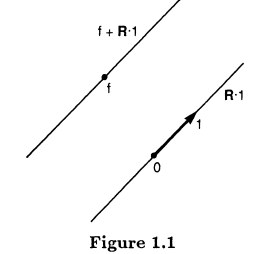
\includegraphics[scale = 0.5]{geo_exp_fam.png}}
\end{minipage}
\caption{\footnotesize{\textbf{The quotient space $\cR_{\cX}/\cR.1$ contains all lines in $\cR_{\cX}$ in parallel to $\cR.1$. \citep{murray1993differential}}}}
\label{fig: geo_exp_fam}
\end{figure}


\item  \begin{proposition} (\textbf{Geometrical criterion for exponential families}) \citep{murray1993differential}\\
$P$ is an affine subspace of $\cP$ generated by a vector space $V \subset \cR_{\cX}/\cR.1$ if and only if $\widetilde{P}$ is an affine subspace of $\cM$ generated by
\begin{align*}
\widetilde{V} = \set{f \in \cR_{\cX}: f+ \cR.1 \in V}
\end{align*} Hence $P$ is an \underline{\textbf{exponential family}} if and only if $\widetilde{P}$ is an \underline{\textbf{affine subspace}} of $\cM$.
 \end{proposition}
 
 \item Since the \emph{\textbf{derivatives of the scores lie in the span of the scores}} at each point is characteristic of affine subspaces, it follows that $P$ is an exponential family, if and only if 
 \begin{align*}
 \widetilde{\ell}_{i,j}(\mb{\eta}) &= \sum_{k=0}^{d}\Gamma_{i,j}^{k}(\mb{\eta})\widetilde{\ell}_{k}(\mb{\eta})
 \end{align*} where $\widetilde{\ell}(\exp(\lambda)p)= \widetilde{\ell}(\mb{\eta}) = \ell(\mb{\eta}) + \lambda$ is the log-likelihood defined via $\widetilde{V}$. Also $\widetilde{\ell}_{0}(\mb{\eta}) = 1$ and $\widetilde{\ell}_{0,j}(\mb{\eta}) = 0$. The linear cooefficients $\Gamma_{i,j}^{k}(\mb{\eta})$ are called the \underline{\emph{\textbf{Christoffel symbol}}}. 
\end{itemize}

\subsection{Computational criterion for exponential families}
\begin{itemize}
\item To show that $\widetilde{P}$ is an affine subspace in $\cM$, it suffices to know if the $\ell_{i,j}$ are in the tangent space to $P$ for each $i, j = 1, \ldots , d$.

\item \begin{definition}
We can define an \underline{\emph{\textbf{inner product}}} in \emph{tangent space} $T_{p}P$ via expectation operation
\begin{align}
\inn{f}{g}_{p} &= \E{p}{f\,g} \label{eqn: inn_prod_exp}
\end{align} on the subspace of $p$ square-integrable random variables $f$, i.e. those random variables satisfying $\E{p}{f^2} < \infty$. 
\end{definition} 

In general it suffices to assume that the \emph{\textbf{scores}} $\widetilde{\ell}_{k}(p)$ at $p$ and the \emph{second derivatives} $ \widetilde{\ell}_{i,j}(p)$ are $p$ square-integrable.

\item \begin{definition}
The \underline{\emph{\textbf{Fisher information matrix}}} is defined as
\begin{align}
g_{i,j}(p):= \inn{\ell_i}{\ell_j}_{p} &= \E{p}{\ell_i\, \ell_j}, \quad \text{for }i,j = 1, \ldots, d. \label{eqn: fisher_info}
\end{align} The Fisher information matrix is just the matrix of the \emph{\textbf{inner product} with respect to the \textbf{basis}} in $T_{p}P$ defined by the scores. It is also called the \underline{\emph{\textbf{first fundamental form}}} of regular surface in differential geometry.
\end{definition}

\item This inner product on $\cR_{\cX}$ defines a \emph{\textbf{normal space}} $N_p$ to $T_{p}\widetilde{P}$ such that
\begin{align}
\cR_{\cX} &= N_p \oplus T_{p}\widetilde{P}. \label{eqn: normal_tangent_decomp}
\end{align} if $f \in \cR_{\cX}$ is a random variable its \emph{\textbf{normal component}} in $N_p$ is
\begin{align}
\Pi_{p}(f) &= f - \sum_{m,n}g^{m,n}\E{p}{f\,\ell_{m}}\,\ell_{n} - \E{p}{f}  \label{eqn: normal_tangent_decomp2}
\end{align} where $g^{m,n}$ is the \emph{\textbf{inverse}} of the Fisher information matrix. 

Note
\begin{align*}
\inn{\Pi_{p}(f)}{1}_{p} &=  \E{p}{f} - \sum_{i,j}g^{i,j}\E{p}{f\,\ell_{i}}\,\E{p}{\ell_{j}} - \E{p}{f} = 0\\
\inn{\Pi_{p}(f)}{\ell_k}_{p} &=  \E{p}{f\,\ell_k} - \sum_{i,j}g^{i,j}\E{p}{f\,\ell_{i}}\,\E{p}{\ell_{j}\ell_k} = \E{p}{f\,\ell_k} - \sum_{i,j}g^{i,j}g_{j,k}\E{p}{f\,\ell_{i}} = 0
\end{align*} where $\E{p}{\ell_{j}} = 0$ for all $j$.

We can rewrite $f$ as
\begin{align*}
f &= (f - \Pi_{p}(f)) + \Pi_{p}(f)
\end{align*} and $ (f - \Pi_{p}(f))$ is a \emph{linear combinations of the scores} and the constant random variables so in $T_{p}\widetilde{P}$.

\item \begin{proposition} (\textbf{Computational criterion for exponential families}) \citep{murray1993differential}\\
The family is \textbf{exponential} if and only if the functions $\ell_{i,j}$ are always tangential to $\widetilde{P}$. This is equivalent to the \textbf{\underline{normal
component} of each $\ell_{i,j}$ vanishing}, that is, to
\begin{align}
\alpha_{i,j}(p) = \Pi_{p}(\ell_{i,j})&=   \ell_{i,j} - \sum_{m,n}g^{m,n}\E{p}{\ell_{i,j}\,\ell_{m}}\,\ell_{n} - \E{p}{\ell_{i,j}}  = 0 \label{eqn: 2nd_fundamental_form} 
\end{align} The quantity $\alpha_{i,j}$ is called the \underline{\textbf{second fundamental form}} of the family. It is also called the \textbf{imbedding curvature} in \citep{amari2007methods}.
 \end{proposition}
 
This proposition states that the \textbf{second fundamental form vanishing} characterises affine subspaces.
 
 \item The \emph{geometric interpretation} for above proposition is the following. $\widetilde{\ell}_{k}$ is tangent to $\widetilde{P}$ and $\widetilde{\ell}_{i,j}$ measures the rate of change of $\widetilde{\ell}_{k}(p)$ as the point $p$ moves around $\widetilde{\cP}$. These changes are to be regarded as due to \emph{two causes}.
\begin{enumerate}
\item The first cause is that the \emph{\textbf{lines}} in $\widetilde{\cP}$ on which the parameters are \emph{constant} may be \textbf{\emph{bending around}};
\item The second cause is that the \textbf{\emph{surface}} $\widetilde{\cP}$ itself may be \emph{\textbf{bending around}} inside $\cM$.
\end{enumerate}  The tangential and normal components of $\widetilde{\ell}_{i,j}$ measure these two types of bending respectively. So the vanishing
of the normal component of $\widetilde{\ell}_{i,j}$ corresponds to the fact that \textbf{the surface $\widetilde{P}$ is not bending}.

\item \begin{definition}
We can define a scalar quanitity $\gamma$ from $\alpha_{i,j}$ so that $\gamma = 0$ if and only if $\alpha_{i,j} = 0$ for all $i,j$. 
\begin{align}
\gamma(p)  &= \sum_{i,j,k,l}g^{i,j}(p)g^{k,l}(p)\E{p}{\alpha_{i,k}(p)\, \alpha_{j,l}(p)} \label{eqn: stats_curvature}
\end{align} where $g^{i,j}$ is the \emph{\textbf{inverse}} of the Fisher information matrix.  The function $\gamma$, in the case of a \emph{one-dimensional family} is Efron's \underline{\emph{\textbf{statistical curvature}}}.
\end{definition} 

Note that since $g^{i,j}$ is positive definite, $\gamma = 0$ if and only if $\alpha_{i,j} = 0$ for all $i,j$.

\item 
\begin{proposition}
The family $P$ is \textbf{exponential} if and only its \textbf{statistical curvature} $\gamma(p) = 0$ for all $p \in P$.
\end{proposition}

This is equivalent to say that the exponential families are \emph{flat}.
\end{itemize}

\subsection{Parameter independence}
In this section, we discuss how $\alpha_{i,j}$ depends on the choice of coordinates. We have \textbf{four equivalent criteria} to decide if a family of probability distribution is exponential. 
\begin{enumerate}
\item The subset of positive measures $\widetilde{\cP}$ is an \emph{\textbf{affine subspace}} in $\cM$;
\item The \emph{second order derivatives} of log-likelihood $\partial_i \partial_j \ell$ are in the span of the \textbf{\emph{scores}} $\set{\partial_i \ell}$ and the constants; 
\item The \emph{\textbf{second fundamental form}} $\alpha_{i,j}$ are vanishing;
\item The \emph{\textbf{statistical curvature}} $\gamma$ is vanishing.
\end{enumerate}

Under reparameterization from $\mb{\eta}$ to $\mb{\theta}$, we compute these quantities. 
\begin{itemize}
%\item We will see that $\gamma$ is a function of $p$ and is not depending on choice of coordinates.
\item
\begin{align}
\frac{\partial^2\ell }{\partial \eta_{i} \partial \eta_{j}} &= \Gamma_{i,j}^{k}\partdiff{\ell}{\eta_{k}} +  \Gamma_{i,j}^{0} \label{eqn: ell_2_linspan_ell_1}
\end{align} Here we use the '\emph{\textbf{Einstein summation convention}}' that any index which occurs \emph{both raised and lowered} is \emph{summed} over. 

If we change coordinates, by the chain rule,
\begin{align}
\partdiff{\ell}{\theta_k} &= \partdiff{\eta_i}{\theta_k}\partdiff{\ell}{\eta_i} \nonumber\\
\partdiff{\ell}{\eta_i} &= \partdiff{\theta_k}{\eta_i}\partdiff{\ell}{\theta_k} \label{eqn: change_of_coordinate_1}
\end{align} and
\begin{align}
\frac{\partial^2\ell}{\partial \theta_k \partial \theta_{l}} &= \frac{\partial^2\eta_i}{\partial \theta_k \partial \theta_{l}} \partdiff{\ell}{\eta_{i}}  + \frac{\partial^2\ell }{\partial \eta_{i} \partial \eta_{j}} \partdiff{\eta_{i}}{\theta_k}\partdiff{\eta_{j}}{\theta_l} \label{eqn: change_of_coordinate_2}
\end{align} Substituting \eqref{eqn: ell_2_linspan_ell_1} and \eqref{eqn: change_of_coordinate_1} into \eqref{eqn: change_of_coordinate_2}, we have 
\begin{align*}
\frac{\partial^2\ell}{\partial \theta_k \partial \theta_{l}} &= \frac{\partial^2\eta_i}{\partial \theta_k \partial \theta_{l}} \partdiff{\ell}{\eta_{i}}  + \frac{\partial^2\ell }{\partial \eta_{i} \partial \eta_{j}} \partdiff{\eta_{i}}{\theta_k}\partdiff{\eta_{j}}{\theta_l} \\
&=  \frac{\partial^2\eta_i}{\partial \theta_k \partial \theta_{l}} \partdiff{\ell}{\eta_{i}}  +  \Gamma_{i,j}^{q}\partdiff{\ell}{\eta_{q}}  \partdiff{\eta_{i}}{\theta_k}\partdiff{\eta_{j}}{\theta_l} +  \Gamma_{i,j}^{0}\partdiff{\eta_{i}}{\theta_k}\partdiff{\eta_{j}}{\theta_l} \\
&= \paren{\frac{\partial^2\eta_i}{\partial \theta_k \partial \theta_{l}} + \Gamma_{m,n}^{i}\partdiff{\eta_{m}}{\theta_k}\partdiff{\eta_{n}}{\theta_l}}\partdiff{\ell}{\eta_{i}} +  \Gamma_{i,j}^{0}\partdiff{\eta_{i}}{\theta_k}\partdiff{\eta_{j}}{\theta_l} \\
&= \paren{\frac{\partial^2\eta_i}{\partial \theta_k \partial \theta_{l}}\partdiff{\theta_r}{\eta_i} + \Gamma_{m,n}^{i}\partdiff{\theta_r}{\eta_i}\partdiff{\eta_{m}}{\theta_k}\partdiff{\eta_{n}}{\theta_l}}\partdiff{\ell}{\theta_{r}} +  \Gamma_{i,j}^{0}\partdiff{\eta_{i}}{\theta_k}\partdiff{\eta_{j}}{\theta_l} \\
\end{align*} Therefore if $\partial_i \partial_j \ell(\mb{\eta})$ are in the span of the scores $\set{\partial_i  \ell(\mb{\eta})}$, so also is $\partial_i \partial_j \ell(\mb{\theta})$.

\item The \emph{second fundamental form} $\alpha_{k,l}$ under  $\mb{\theta}$ can be computed by considering it as the projection of $\frac{\partial^2\ell}{\partial \theta_k \partial \theta_{l}}$ to the orthogonal space of $T_{p}\widetilde{P} = \text{span}\set{\partial_i  \ell(\mb{\eta})}$. 
\begin{align}
\alpha_{k,l} &= \Pi\paren{\frac{\partial^2\ell}{\partial \theta_k \partial \theta_{l}} } \nonumber\\
&= \Pi\paren{ \frac{\partial^2\ell }{\partial \eta_{i} \partial \eta_{j}} \partdiff{\eta_{i}}{\theta_k}\partdiff{\eta_{j}}{\theta_l} }= \Pi\paren{ \frac{\partial^2\ell }{\partial \eta_{i} \partial \eta_{j}}} \partdiff{\eta_{i}}{\theta_k}\partdiff{\eta_{j}}{\theta_l} \nonumber\\
&= \alpha_{i,j} \partdiff{\eta_{i}}{\theta_k}\partdiff{\eta_{j}}{\theta_l}  \label{eqn: 2nd_fundamental_form_change_coordinate}
\end{align} The second equation holds since $ \Pi\paren{\partdiff{\ell}{\eta_{i}}} = 0$. It follows that $\alpha_{k,l}$ vanishes precisely when $\alpha_{i,j}$ vanishes.

\item Note that the \emph{\textbf{Fisher information matrix}} under \emph{\textbf{reparameterization}} $\mb{\theta}$ can be computed as
\begin{align}
g_{k,l}(\mb{\theta}) &=\E{p}{\frac{\partial^2\ell}{\partial \theta_k \partial \theta_{l}} } \nonumber\\
&= \frac{\partial^2\eta_i}{\partial \theta_k \partial \theta_{l}}\E{p}{ \partdiff{\ell}{\eta_{i}}}  + \E{p}{\frac{\partial^2\ell }{\partial \eta_{i} \partial \eta_{j}}} \partdiff{\eta_{i}}{\theta_k}\partdiff{\eta_{j}}{\theta_l} \nonumber\\
&= g_{i,j}(\mb{\eta})\; \partdiff{\eta_{i}}{\theta_k}\partdiff{\eta_{j}}{\theta_l} \label{eqn: fisher_info_change_coordinate}
\end{align} since $\E{p}{ \partdiff{\ell}{\eta_{i}}} = 0$ for all $i$.

From \eqref{eqn: fisher_information_partition_second_order}, we see that the \emph{\textbf{intrinsic properties}} of curvature are \emph{\textbf{unchanged}} under different parametrizations. In general, the Fisher information matrix provides a \underline{\emph{\textbf{Riemannian metric}}} (more precisely, the Fisher-Rao metric) for the manifold of thermodynamic states.


\item Substituting results in \eqref{eqn: 2nd_fundamental_form_change_coordinate} and \eqref{eqn: fisher_info_change_coordinate} into \eqref{eqn: stats_curvature}, we see that the Jacobians are all cancelled out. The following proposition readily follows:
\begin{proposition}
\underline{The statistical curvature $\gamma$ is an \textbf{invariant}} of the family of distributions $P$. That is, it is a function on $P$ that is \textbf{independent} of the choice of coordinates. 
\end{proposition}

\item From the proposition above, we see that both the  geometric criterion (\emph{affine subspace}) and the computational criterion (\emph{vanishing statistical curvature}) for \emph{exponential families} are \textbf{independent} of choice of coordinates. 
\end{itemize}


\newpage
\bibliographystyle{plainnat}
\bibliography{book_reference.bib}
\end{document}